% Problem Statement
\chapter{Problem Statement} \label{sec:problem}
% TODO describe on high level the two problems

\section{Onboard Human Pilot and Full-State Feedback Adaptive Control}
% TODO change "in this paper" to "in this thesis"
% TODO bring notation in line with MIMO example

%We consider linear single-input, states-accessible plant models of the form 
%\begin{equation}
%\dot x_p = A_p x_p + B_p u_p	
%\end{equation}

A Model Reference Adaptive Control (MRAC)-based adaptive autopilot is capable of addressing anomalies that can be represented as parametric uncertainties, but may perform poorly when an anomaly causes the order of the vehicle dynamics to change \cite{narendra2012stable, lavretsky2013robust}. A human pilot flying manually may detect such an anomaly and adapt to the anomalous dynamics, but the pilot's tracking performance may be noticeably poorer after a change in dynamics and pilot adaptation \cite{hess2015modeling, zaal2016manual}. Our goal in this paper is to combine the actions of an adaptive autopilot with those of a human pilot and apply the resulting shared controller to two such anomalies, one representing a physical actuator fault and the other a cyber attack on the vehicle's sensors. We focus on the lateral-directional dynamics of a fixed-wing aircraft, which are described briefly. For an aircraft trimmed in straight and level flight with equilibrium speed $u_0$ and pitch angle $\theta_0$, and assuming small perturbations about the equilibrium point, the lateral-directional dynamics of the aircraft can be linearized to the form $\dot{x}_{\mathrm{lat}} = A_{\mathrm{lat}} x_{\mathrm{lat}} + B_{\mathrm{lat}} u_{\mathrm{lat}}$ where
\begin{eqnarray}
	x_{\mathrm{lat}} &=& \begin{bmatrix}\beta & p_s & \phi_s & r_s \end{bmatrix}^T, \qquad u_{\mathrm{lat}} = \begin{bmatrix}\delta_r & \delta_a \end{bmatrix}^T \nonumber \\
	A_{\mathrm{lat}} &=& \begin{bmatrix}
			\frac{Y_\beta}{u_0} & \frac{Y_p}{u_0} & \frac{g_0\cos{\theta_0}}{u_0} & \frac{Y_r}{u_0} - 1 \\
			L_\beta & L_p & 0 & L_r \\
			0 & 1 & 0 & 0 \\
			N_\beta & N_p & 0 & N_r
		\end{bmatrix}, \qquad B_{\mathrm{lat}} = \begin{bmatrix}
			\frac{Y_{\delta_r}}{u_0} & \frac{Y_{\delta_a}}{u_0} \\
			L_{\delta_r} & L_{\delta_a} \\
			0 & 0 \\
			N_{\delta_r} & N_{\delta_a} 
		\end{bmatrix}
\end{eqnarray}
\noindent with definitions of the stability and control derivatives in matrices $A_{\mathrm{lat}}$ and $B_{\mathrm{lat}}$ skipped for brevity (see Ref.~\cite{lavretsky2013robust} for more details). The states correspond to sideslip angle, stability axis roll rate, stability axis bank angle, and stability axis yaw rate, respectively, while the control inputs correspond to rudder and aileron deflections.

Approximate second-order linearized rolling mode dynamics are extracted from this fourth-order system, and this system is given by
\begin{equation}
	\underbrace{\begin{bmatrix}
			\dot{\phi} \\ \dot{p}
		\end{bmatrix}}_{\dot{x}_p} = \underbrace{\begin{bmatrix}
			0 & 1 \\ 0 & L_p
		\end{bmatrix}}_{A_p} \underbrace{\begin{bmatrix}
			\phi \\ p
		\end{bmatrix}}_{x_p} + \underbrace{\begin{bmatrix}
			0 \\ L_{\delta_a}
		\end{bmatrix}}_{B_p} \delta_a
	\label{eqn:2nd_order_lateral}
\end{equation} \noindent with an open-loop transfer function
\begin{equation}
		\frac{\Phi(s)}{\Delta_a(s)} = \frac{L_{\delta_a}}{s^2 - L_p s}
\end{equation}

In these equations, $\delta_a$ represents aileron input, and $\phi$ and $p$ denote the aircraft bank angle and roll rate in stability axes, with the subscript $(\cdot)_s$ dropped for notational simplicity. It is assumed that the states ($x_p$) are fully available for feedback (directly from sensors for $p$, and via integration of $p$ for $\phi$). $L_p$ is the roll damping derivative and $L_{\delta_a}$ is the rolling moment due to aileron deflection. We consider scenarios in which these parameters may be unknown, but are addressed in normal operation by an MRAC-based adaptive autopilot. The system has been simplified by fixing $\delta_r(t) = 0$ (no rudder input), so that aileron deflection is the only input. In normal operation, we assume the vehicle has sufficiently fast actuators, so that $\delta_a(t) = u(t)$ and equivalently $\Delta_a(s) = U(s)$, where $u(t)$ is the control signal. 

We now introduce two anomalies into the problem where the first, denoted as case (i), consists of a change in the actuator dynamics, represented as a change in the actuator model from a gain to a first-order lag. The second anomaly, denoted as case (ii), is a latency introduced between sensing and actuation, which may be the result of a denial-of-service (DOS) cyber attack. 
%Two anomalous scenarios are presented (i) where the ailerons become sluggish, represented as a change in the actuator model from a gain to a first-order lag, and (ii) where there is a significant delay between the time the measurements are taken to the time of actuation. Both of these anomalies may occur due to cyber physical failures.

\subsection{Actuator Fault}
An anomaly is introduced which changes the actuator dynamics from a gain to a first-order lag
\begin{equation}
	\frac{\Delta_a(s)}{U(s)} = \begin{cases}
		\hfil 1 & t < t_{s,p}\\
		\frac{1}{T_l s + 1} & t \geq t_{s,p}
	\end{cases} 
	\label{eqn:actuator_dynamics_symbolic}
\end{equation} 
\noindent so that the dynamics of the rolling mode change suddenly from second-order (\ref{eqn:2nd_order_lateral}) to third-order (\ref{eqn:plant_3_symbolic}).
\begin{equation}
	\underbrace{\begin{bmatrix}
		\dot{\phi} \\ \dot{p} \\ \ddot{p}
	\end{bmatrix}}_{\dot{x}_p'} = \underbrace{\begin{bmatrix}
		0 & 1 & 0\\ 0 & 0 & 1 \\ 0 & \frac{L_p}{T_l} & L_p - \frac{1}{T_l}
	\end{bmatrix}}_{A_p'} \underbrace{\begin{bmatrix}
		\phi \\ p \\ \dot{p}
	\end{bmatrix}}_{x_p'} + \underbrace{\begin{bmatrix}
		0 \\ 0 \\ \frac{L_{\delta_a}}{T_l}
	\end{bmatrix}}_{B_p'} u
	\label{eqn:plant_3_symbolic}
\end{equation}

If the change in the order of the plant is not known to the adaptive controller, it may no longer be possible for it to stabilize the aircraft following such a change. The question then is if shared control with suitable input from the pilot leading to feedback on $\dot{p}$ can result in improved performance.
%If the angular acceleration is available for measurement, the resulting problem can be viewed as the adaptive control of a third-order plant whose states are all accessible.

\subsection{Time-Delayed Sensor Measurements}
We consider a cyber-physical anomaly, such as a DOS-type cyber attack, which leads to latency between sensor measurements and actuation. We model this anomaly as the addition of a time delay $\tau$ of the state measurements before the computation of the control input. We approximate the corresponding transfer function of a pure time delay $\tau$ as a first-order filter
\begin{equation}
	e^{-\tau s} \approx \frac{1}{1 + \tau s}
	\label{first_order_delay_approx}
\end{equation}

We note that the resulting approximation of delayed plant dynamics is third-order 
\begin{equation}
	\underbrace{\begin{bmatrix}
		\dot{\phi} \\ \dot{p} \\ \ddot{p}
	\end{bmatrix}}_{\dot{x}_\sigma'} = \underbrace{\begin{bmatrix}
		0 & 1 & 0\\ 0 & 0 & 1 \\ 0 & \frac{L_p}{\tau} & L_p - \frac{1}{\tau}
	\end{bmatrix}}_{A_\sigma'} \underbrace{\begin{bmatrix}
		\phi \\ p \\ \dot{p}
	\end{bmatrix}}_{x_\sigma'} + \underbrace{\begin{bmatrix}
		0 \\ 0 \\ \frac{L_{\delta_a}}{\tau}
	\end{bmatrix}}_{B_\sigma'} u
	\label{eqn:plant_3_tau}
\end{equation}
\noindent where the notation $(\cdot)_\sigma$ denotes the autopilot-sensed (delayed) state. A shared control solution to the anomaly of case (i) can therefore potentially be applied in this case as well.



\section{Remote Human Operation and Output Feedback Adaptive Control}
We consider linear multi-input multi-output (MIMO) plant models of the form
\begin{equation}
\begin{gathered}
\dot x_p = (A_p + B_p \Theta_p^T) x_p + B_p \Lambda_p u_p \\
y_p = C_p x_p, \qquad z_p = C_{pz} x_p \label{eq:plant_dynamics}
\end{gathered}
\end{equation}
where uncertain dynamics lead to the introduction of unknown $\Theta_p$ and $\Lambda_p$ in the plant model, $y_p$ are measurement outputs, and $z_p$ are regulated outputs which we would like to follow prescribed commands. It is assumed that the matrix $CB$ has full rank, and thus the plant has uniform relative degree one (see \cite{qu2016adaptive}). In addition to the dynamics (\ref{eq:plant_dynamics}), the plant's actuators have the first-order dynamics
\begin{equation}
	\dot{u}_p + (D_1 + \Theta_1^T) u_p = D_1 u \label{eq:first_order_act}
\end{equation}
where $D_1$ is a diagonal matrix representing nominal actuator parameters and $\Theta_1$ models uncertainty in the actuator dynamics. 
%Model reference adaptive control (MRAC) with output feedback and closed-loop reference models, such as the method of \cite{qu2016adaptive}, can achieve asymptotic tracking and guarantee stability for this control problem. 

\subsection{Actuator Fault}
Consider the occurrence of an anomaly which causes a sudden change in actuator dynamics from (\ref{eq:first_order_act}) to the second-order model
\begin{equation}
	\ddot{u}_p + (D_2 + \Theta_2^T) \dot{u}_p + (D_1 + \Theta_1^T) u_p = D_1 u. \label{eq:second_order_act}
\end{equation}
This change in dynamics means that the the structure of the model used for control design is no longer accurate, and the autonomous controller may lose stability and command tracking ability.

In addition to an autonomous controller which generates control input $u(t)$ in (\ref{eq:first_order_act}) and (\ref{eq:second_order_act}), a human supervisor is tasked with the high-level operation of the plant (\ref{eq:plant_dynamics}), including mission and task planning (commanding its mode of operation) and monitoring to ensure safe and anomaly-free operation. In this paper, we consider \textit{remote} human operators who cannot sense the vehicle state and dynamics directly through vestibular pathways. The human supervisor may be responsible for the supervision of multiple plant instances, as illustrated in Fig. \ref{fig:uav_supervisor} for the case of HALE VFA platforms. Operation is thus \textit{human-on-the-loop} as opposed to \textit{human-in-the-loop}, as the operator has no role in feedback control. 

\begin{figure}[htbp]
	\centering
	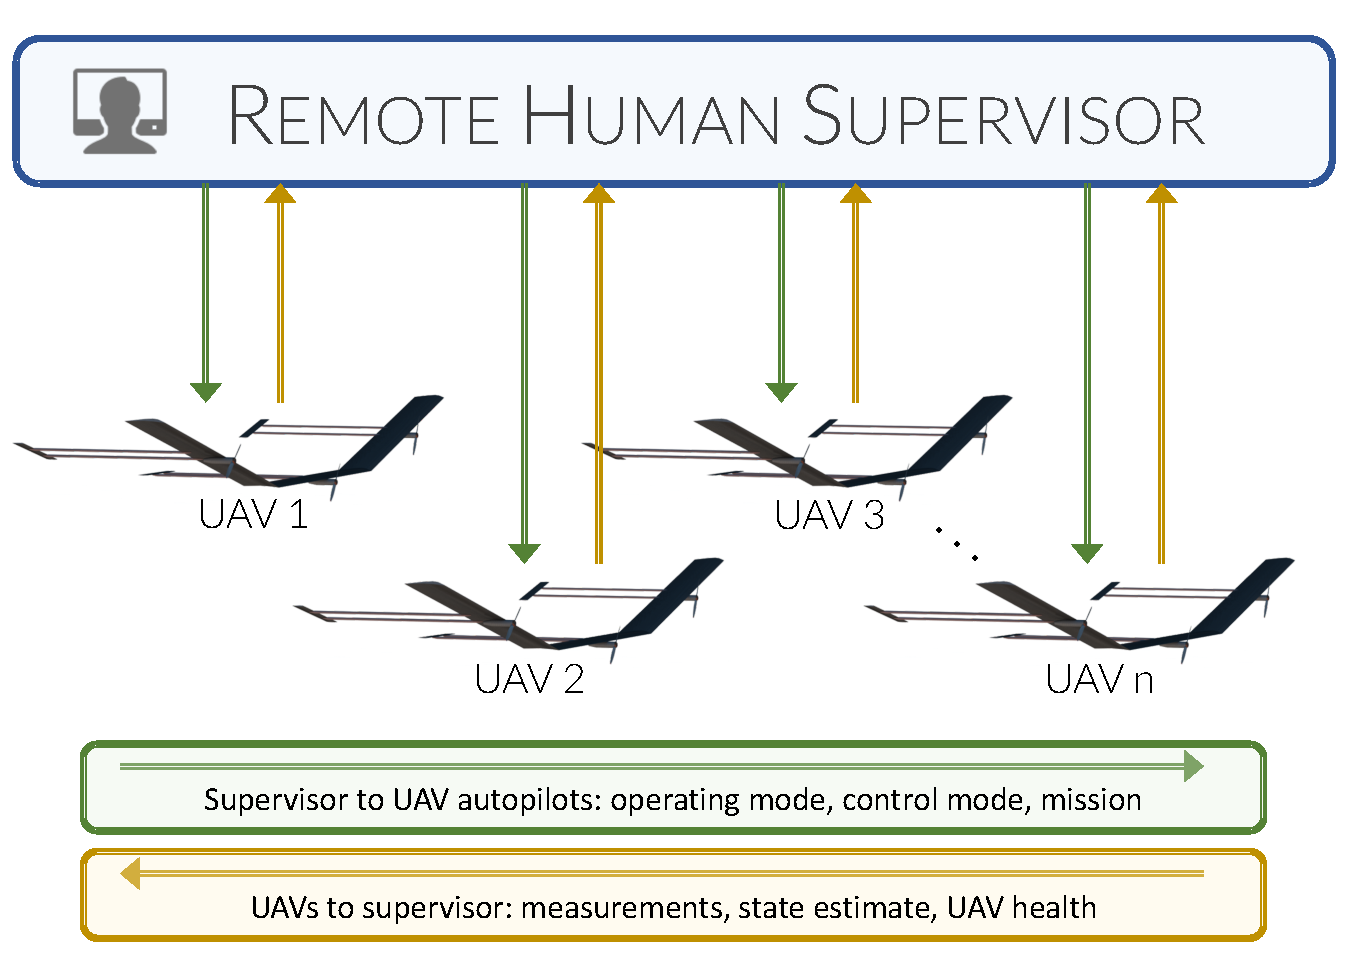
\includegraphics[width=0.95\columnwidth]{uav_supervisor.pdf}
	\caption{Supervisory operation of a fleet of HALE UAVs}
	\label{fig:uav_supervisor}
\end{figure}

The remote human supervisor has information on plant sensor measurements, state estimate, tracking performance, and health (via visual, haptic, and/or auditory interfaces). \textit{Human-in-the-loop} operation is possible via remote controls, allowing the operator to actuate the plant by manually providing $u(t)$ in (\ref{eq:first_order_act}) and (\ref{eq:second_order_act}). The sensing and actuation by the remote human supervisor include time delays $\tau_s, \tau_a > 0$, respectively.

The problem we investigate is whether we can use a suitable combination of 
\begin{enumerate}[label=(\alph*)]
	\item autonomous control methodologies
	\item a remote human supervisor
\end{enumerate}
  to successfully mitigate the anomalous dynamics (\ref{eq:second_order_act}) and restore tracking performance in the presence of uncertainty. We refer to this class of anomaly response as a shared control response. This work builds on anomaly response frameworks using adaptive autopilots and on-board human pilots reported in \cite{farjadian2017bumpless} and \cite{thomsen2018shared}.
